\documentclass[crop,tikz]{standalone}
\usepackage[subpreambles=true]{standalone}

../presentation_7_30_18/preamble.tex

\begin{document}

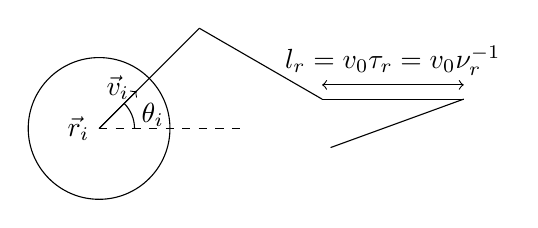
\begin{tikzpicture}[scale=0.9]
\draw (0, 0) circle (1) node[left]{$\vec{r}_i$};
\draw[dashed] (0, 0) -- (2, 0);
\draw (0, 0) -- (1.4142135623730951, 1.4142135623730951);
\draw (0, 0)[->] -- (0.5303300858899107, 0.5303300858899107) node[midway, above]{$\vec{v}_i$};
\draw (0.5, 0) arc (0:45:0.5) node[midway, right]{$\theta_i$};
\draw (1.4142135623730951, 1.4142135623730951) -- (3.1462643699419726, 0.41421356237309503);
\draw (3.1462643699419726, 0.41421356237309503) -- (5.1462643699419726, 0.41421356237309503);
\draw[<->] (3.1462643699419726, 0.61421356237309503) -- (5.1462643699419726, 0.61421356237309503) node[midway, above]{$l_r = v_0\tau_r = v_0\nu_r^{-1}$};
\draw (5.1462643699419726, 0.41421356237309503) -- (3.2668791283701557, -0.26982672427824277);
\end{tikzpicture}

\end{document}
